\usepackage{ifthen}
\usepackage{float}
\usepackage{calc}
\usepackage[export]{adjustbox}% http://ctan.org/pkg/adjustbox
\usepackage{xstring}
\usepackage{multicol}
\usepackage[framemethod=TikZ]{mdframed}

% Extract a symbol from the ISO document. And show it together with the title and warning text.
%
% Params:		Page with the symbol on it.
%			Title
%			Warning text
%			Y height on the page.
%
\newcommand{\decal}[5]{
\begin{minipage}{\linewidth}
	\begin{minipage}[t]{0.3\textwidth}
	       \vspace{0pt}
	       % The ISO document has a 'gutter' - so we shift the X a bit on the left/right page.
	       %
		\ifthenelse{\isodd{#1}}{
			\includegraphics[width=0.9\textwidth,page=#1,viewport=103 #3 291 #4,clip=true]{13GR_PistopioimeniSimansi_ISO_7010.pdf}
		}{
			\includegraphics[width=0.9\textwidth,page=#1,viewport=70 #3 261 #4,clip=true]{13GR_PistopioimeniSimansi_ISO_7010.pdf}
		}
	\end{minipage}
	\begin{minipage}[t]{0.6\textwidth}
		\setlength{\parindent}{4em}
		\setlength{\parskip}{1.2em}
	       \vspace{0pt}\raggedright
		{\LARGE \textbf{#2}}
	
		#5
		\vspace{0.5cm}
	\end{minipage}
\end{minipage}
}

% Turns out that the symbols are a bit shifted in the Y position or size depending on what
% class they are. So we split them into the three sections that have height differences.
%
% Params:		Page with the symbol on it.
%			Title
%			Warning text
%
\newcommand{\action}[3]{\decal{#1}{#2}{520}{715}{#3}}
\newcommand{\prohib}[3]{\decal{#1}{#2}{495}{690}{#3}}
\newcommand{\warn}[3]{\decal{#1}{#2}{520}{715}{#3}}

% A full page with a machine on it.
%
% Params:		Machine name
%			Tokens for standard instrutions: Zero or more from
%				Approval		Trustee approval needed.
%				Noise		Not after 19:00
%				Two			Two people required
%				Log			use must be logged
%				Dewalt		Attach dewalt dutch extractor.
%			Specific instructions 
%			Warnings, Symbols
%			Extra footer/bottom of the page text
%
\newcommand{\machinePage}[5]{%
\begin{center}
	\vspace{0cm}
	{\fontsize{50}{60} \textbf{#1}}
 
	\action{49}{%
		\textbf{%
 		\IfSubStr{#2}{Approval}%
			{Instructions \& Approval Mandatory}
			{\IfSubStr{#2}{NoMandatory}{Mandatory Safety Rules}{Instruction Mandatory}}%
		}}
		{%
		\IfSubStr{#2}{NoMandatory}{}{Instruction \textbf{prior} to use is \textbf{mandatory}. Check the wiki for who can help you.}
		\IfSubStr{#2}{Approval}{You must also have a `\textbf{dangerous equipment waiver}' filed with the foundations trustees and been given \textbf{approval or card access} to use the machine.}{}
			
		#3

		\IfSubStr{#2}{Noise}{\smallicontext{\seventoseven}{
			Machine can only be used between 07:00 - 19:00 (be kind to our neighbours)
			}
		}{}

		\IfSubStr{#2}{Two}{\smallicontext{\twopersons}{A second person must be present during operation, have agreed to be your second, knows how to stop the machine and what to do in an emergency.	}
		}{}

		\IfSubStr{#2}{Log}{Report any use in the log - and \textbf{pay for it}!}{}

		\IfSubStr{#2}{Dewalt}{Be sure to attach and power on the dust extractor.}{}
	}
	\begin{multicols}{2}#4\end{multicols}
	
	\vspace{0.2cm}
	#5

	If a machine is not clean or appears broken - then report this to the mailing list. Clean/fix prior to use.

	\textbf{Report any damage, issues or accident within 24 hours to the mailing list.}
\end{center}
\vfill
\begin{flushright}
{\tiny \version -- \today}
\end{flushright}
\pagebreak
}
\newcommand{\smallicontext}[2]{%
\begin{mdframed}[roundcorner=4pt] 
\begin{tabular}{lp{0.8\linewidth}}
#1 & #2 \\
\end{tabular}
\end{mdframed}
}

% Two person symbol
\newcommand{\twopersons}{
\raisebox{-.5\height}{\includegraphics[width=6mm]{File:Aiga_toiletsq_men}}\textbf{x 2} 
}

\newcommand{\seventoseven}{
\raisebox{-.5\height}{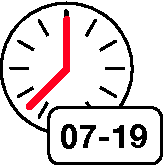
\includegraphics[width=10mm]{clock-limits}}
}




